\documentclass[aspectratio=169]{beamer}
\usetheme{Madrid}
\usecolortheme{default}
\setbeamertemplate{navigation symbols}{}
\setbeamertemplate{footline}[frame number]
\usepackage[gen]{eurosym}
\usepackage{graphicx}
\usepackage{tikz}
\usepackage{ragged2e}
\usepackage{booktabs}
\usepackage{array}
\usepackage{pifont}
\usepackage{multicol}
\newcommand{\imgsource}[1]{\vspace{0.3em}\tiny\color{gray}{#1}}
\setbeamerfont{note page}{size=\small}
\title{Operations-Driven Analytics in E-Commerce}
\subtitle{First Approach}
\author{Loris Emanuelli}
\institute{Capstone Projects 121 \& 122 (2025--2026)}
\date{}

\begin{document}

{
\usebackgroundtemplate{\includegraphics[width=\paperwidth,height=\paperheight]{img_ecommerce_hero.jpg}}
\begin{frame}[plain]
    \color{white}
    \begin{tikzpicture}[remember picture,overlay]
        \node[anchor=south west,xshift=0.9cm,yshift=0.9cm] (titleblock) {\begin{minipage}{0.62\textwidth}
            \LARGE \textbf{Operations-Driven Analytics in E-Commerce}\\[0.5em]
            \large First Approach
        \end{minipage}};
        \node[anchor=north west,xshift=0.9cm,yshift=-0.4cm] at (titleblock.south west) {\begin{minipage}{0.6\textwidth}
            \small Loris Emanuelli\\
            Capstone Projects 121 \& 122 (2025--2026)
        \end{minipage}};
    \end{tikzpicture}
    \imgsource{Source: Unsplash}
    \note{Welcome everyone, open with the flash sale vignette, and position this as the first exploratory checkpoint for Team 121.}
\end{frame}
}
\usebackgroundtemplate{}

\begin{frame}{Today's Journey}
    \begin{columns}[T,onlytextwidth]
        \column{0.55\textwidth}
        \begin{enumerate}[1.]
            \item Set the opening scene and objectives
            \item Link analytics to operations leverage
            \item Surface review paper takeaways
            \item Demystify the Newsvendor logic
            \item Map relevance, gaps, and risks
            \item Align on datasets, next moves, and discussion
        \end{enumerate}
        \column{0.4\textwidth}
        \centering
        \includegraphics[width=\linewidth]{img_data_dashboard.jpg}
        \imgsource{Source: Unsplash}
    \end{columns}
    \note{Preview the flow so the audience knows we will move from context, through literature and the model, toward application and open questions.}
\end{frame}

\begin{frame}{Responsive Inventory in Motion}
    \begin{columns}[c,onlytextwidth]
        \column{0.52\textwidth}
        \justifying
        Mi\v{s}i\'{c} \& Perakis (2020) document how retailers fuse POS, clickstream, and supplier telemetry to shrink the latency between demand sensing and replenishment. Their case analyses show safety-stock reductions of 15--25\% once inventory targets refresh with real-time signals across stores and DCs.
        \vspace{0.8em}
        \begin{block}{Signals Highlighted in the Review}
            \begin{itemize}
                \item SKU-level velocity forecasts updated from streaming data
                \item Reverse logistics information feeding net-demand estimates
                \item Supplier reliability scores guiding multi-echelon positioning
            \end{itemize}
        \end{block}
        \vspace{0.4em}
        \footnotesize\textit{Mi\v{s}i\'{c} \& Perakis (2020), Sections 3.1--3.2}
        \column{0.44\textwidth}
        \centering
        \includegraphics[width=\linewidth]{img_fulfillment.jpg}
        \imgsource{Source: Unsplash}
    \end{columns}
    \note{Explain how the review highlights adaptive inventory policies; tie to our need to quantify variability across e-commerce channels.}
\end{frame}

\begin{frame}{Last-Mile Orchestration}
    \begin{columns}[T,onlytextwidth]
        \column{0.48\textwidth}
        \begin{block}{Control Tower Actions}
            \begin{itemize}
                \item Predict route saturation by lane and time window
                \item Re-sequence stops when telemetry flags bottlenecks
                \item Sync promised slots with capacity forecasts
            \end{itemize}
        \end{block}
        \column{0.48\textwidth}
        \begin{exampleblock}{Analytics Payoff}
            \justifying
            The review cites same-day pilots in North America and Asia where integrating vehicle tracking, order forecasts, and workforce data trimmed late deliveries by 12--18\% while containing surge labor. These examples underscore the value of feedback loops that tighten the promise-to-fulfillment cycle.
        \end{exampleblock}
        \vspace{0.4em}
        \footnotesize\textit{Mi\v{s}i\'{c} \& Perakis (2020), Section 3.4}
    \end{columns}
    \note{Reinforce that last-mile responsiveness hinges on analytics loops pulling telemetry from the field and feeding it into promise windows.}
\end{frame}

\begin{frame}{Revenue Management Playbook}
    \justifying
    Mi\v{s}i\'{c} \& Perakis (2020) argue that revenue analytics succeeds when pricing, assortment, and inventory share a common demand backbone. They highlight e-commerce cases where Bayesian or reinforcement learning models update price ladders daily while honoring inventory guardrails.
    \vspace{0.8em}
    \begin{enumerate}
        \item \textbf{Dynamic Pricing:} Learning-based engines respond to elasticity signals while preserving minimum inventory buffers.
        \item \textbf{Assortment Tuning:} Stochastic programs allocate digital shelf space across substitutes using margin and supply risk inputs.
        \item \textbf{Targeted Promotions:} Uplift models prioritize segments that marketing can serve without overwhelming fulfillment capacity.
    \end{enumerate}
    \vspace{0.4em}
    \footnotesize\textit{Mi\v{s}i\'{c} \& Perakis (2020), Sections 4.1--4.3}
    \note{Highlight how revenue levers and operational constraints interact, pointing to the need for shared data between pricing, merchandising, and fulfillment teams.}
\end{frame}

\begin{frame}{Newsvendor Intuition}
    \begin{quotation}
        \justifying
        ``The single-period inventory problem is a balancing act between disappointing customers today and holding excess stock tomorrow. The Newsvendor model quantifies that trade-off so planners can align service levels with risk tolerance.''
    \end{quotation}
    \vspace{0.6em}
    \begin{itemize}
        \item Underage cost ($C_u$) = contribution margin + customer impact.
        \item Overage cost ($C_o$) = holding, markdown, or salvage gap.
        \item Critical fractile balances the two and sets the service target.
    \end{itemize}
    \note{Use the quote to anchor the intuition before moving to formulas, emphasizing the qualitative trade-off stakeholders feel every promotion.}
\end{frame}

\begin{frame}{Newsvendor Mechanics}
    \begin{block}{Critical Fractile Rule}
        \[
            q^\ast = F^{-1}\!\left(\frac{C_u}{C_u + C_o}\right)
        \]
    \end{block}
    \vspace{0.6em}
    \begin{itemize}
        \item $F(q)$: forecast distribution for the selling window.
        \item $C_u$: cost of an unmet unit of demand.
        \item $C_o$: cost of a leftover unit.
        \item Service level target = $\frac{C_u}{C_u + C_o}$.
    \end{itemize}
    \note{Walk through each term, ensuring the audience sees how the cost ratio maps directly to an order quantity via the inverse CDF.}
\end{frame}

\begin{frame}{Flash Sale Example}
    \justifying
    Limited-edition gadget drop, priced at \euro{}120 with a supplier cost of \euro{}70 and liquidation value of \euro{}40.
    \vspace{0.6em}
    \begin{table}[h!]
        \centering
        \begin{tabular}{>{\raggedright\arraybackslash}p{0.52\textwidth} >{\raggedleft\arraybackslash}p{0.35\textwidth}}
            \toprule
            Underage cost $C_u$ (lost margin) & \euro{}50 \\
            Overage cost $C_o$ (liquidation gap) & \euro{}30 \\
            Demand forecast & Normal$(900, 180)$ \\
            Critical fractile & $50/(50+30) = 0.625$ \\
            Optimal order $q^\ast$ & $\approx 958$ units \\
            \bottomrule
        \end{tabular}
    \end{table}
    \vspace{0.5em}
    \begin{itemize}
        \item Decision: order 958 units to balance stockout risk and overage cost.
        \item Interpretation: target a 62.5\% service level for this promotion.
    \end{itemize}
    \note{Step through the arithmetic live so stakeholders see how the numbers tie out and can visualize using the same logic for their SKUs.}
\end{frame}

\begin{frame}{From Model to Decisions}
    \centering
    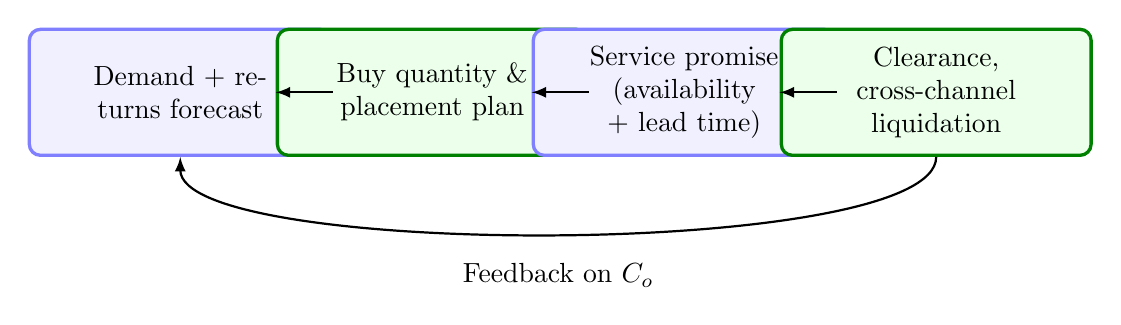
\begin{tikzpicture}[node distance=3.2cm,>=latex]
        \tikzstyle{stage}=[rectangle, rounded corners, draw=blue!50, very thick, text width=3.6cm, align=center, minimum height=1.6cm, fill=blue!6]
        \tikzstyle{action}=[rectangle, rounded corners, draw=green!50!black, very thick, text width=3.7cm, align=center, minimum height=1.6cm, fill=green!8]
        \node[stage] (forecast) {Demand + returns forecast};
        \node[action,right of=forecast] (inventory) {Buy quantity \&\\placement plan};
        \node[stage,right of=inventory] (promise) {Service promise \\ (availability + lead time)};
        \node[action,right of=promise] (liquidation) {Clearance,\\cross-channel liquidation};
        \draw[->,thick] (forecast) -- (inventory);
        \draw[->,thick] (inventory) -- (promise);
        \draw[->,thick] (promise) -- (liquidation);
        \draw[->,thick] (liquidation.south) .. controls +(0,-1.3) and +(0,-1.3) .. (forecast.south) node[midway,below,yshift=-0.25cm]{Feedback on $C_o$};
    \end{tikzpicture}
    \note{Explain how outputs of the Newsvendor logic cascade into placement and promise decisions, with liquidation performance feeding back into future cost estimates.}
\end{frame}

\begin{frame}{Out of Scope Today}
    \begin{alertblock}{Topics Parked for Later Deep Dives}
        \begin{itemize}
            \item Feature-rich demand forecasting and machine learning pipelines
            \item Customer-level uplift modeling for personalization
            \item Automated parameter learning for $C_u$ and $C_o$
        \end{itemize}
    \end{alertblock}
    \vspace{0.6em}
    \begin{block}{Preview}
        These advanced methods will enrich the inputs to our classical models once we establish the baseline decisions and data flows.
    \end{block}
    \note{Clarify the intentional boundary so expectations stay aligned and stakeholders know advanced analytics will follow after the foundational work.}
\end{frame}

\begin{frame}{Where the Model Strains}
    \begin{description}
        \item[Demand shocks] Seasonality and trend breaks can render $F(q)$ obsolete overnight.
        \item[Cost opacity] Loyalty erosion and brand damage are tough to price into $C_u$.
        \item[Portfolio coupling] Shared capacity across SKUs violates the single-period assumption.
        \item[Data hygiene] Returns data and lead times require ongoing cleansing to stay credible.
    \end{description}
    \note{Share these caveats candidly to encourage a culture of stress testing and transparent assumptions.}
\end{frame}

\begin{frame}{Datasets We Are Scoping}
    \begin{table}[h!]
        \centering
        \begin{tabular}{>{\raggedright\arraybackslash}p{0.36\textwidth} >{\raggedright\arraybackslash}p{0.52\textwidth}}
            \toprule
            Dataset & Use Case \\
            \midrule
            JD.com flash sale records & Demand and fulfillment volatility during high-pressure events \\
            Amazon last-mile routing benchmarks & Link delivery promise to actual route constraints \\
            Retail returns and refurbishment logs & Quantify net demand after returns and salvage value \\
            Promotion calendar + fulfillment metrics & Calibrate $C_u / C_o$ under different campaign types \\
            \bottomrule
        \end{tabular}
    \end{table}
    \note{Tie each dataset to the analytical decisions we aim to support, so sponsors see why access matters.}
\end{frame}

{
\usebackgroundtemplate{\includegraphics[width=\paperwidth,height=\paperheight]{img_team.jpg}}
\begin{frame}[plain]
    \color{white}
    \begin{minipage}{0.65\textwidth}
        \LARGE \textbf{Closing \& Discussion}\\[0.6em]
        \large Operations analytics bridges insight and action.\\[0.4em]
        \large Continued collaboration will shape our next iteration.\\[1em]
        \normalsize Thank you for your partnership.
    \end{minipage}
    \imgsource{Source: Unsplash}
    \note{Reiterate the key message, share the collaboration note, and thank the audience.}
\end{frame}
}
\usebackgroundtemplate{}

\begin{frame}{References}
    \begin{itemize}
        \item Velibor V. Mišić \& Georgia Perakis, ``Data Analytics in Operations Management: A Review,'' \emph{Manufacturing \& Service Operations Management}.
        \item Wikipedia, ``Newsvendor model,'' \url{https://en.wikipedia.org/wiki/Newsvendor_model}.
        \item ``Capstone Projects 121 \& 122 2025--2026 Main Doc and Resources.''
    \end{itemize}
    \note{Point the audience to the sources and mention they will also appear in the written submission.}
\end{frame}

\end{document}
